
\documentclass[a4paper,11pt]{article}
\usepackage{Sweave}
\title{Project Parallel Programming \\ MPI All-pair Shortest Path}
\author{ Linus Schoemaker (lsr450/1961667)}
\begin{document}

\maketitle

\section{Introduction}

This report describes the parallel implementation of the All-pairs Shortest Path (ASP) algorithm, using the C MPI-library and the DAS4 cluster computer. 
First we will explain the sequential algorithm. Then we will describe the changes made in order to run this algorithm in parallel. We will also give a theoretical estimation of possible speedup.
In the third section we will show the speed-up achieved by parallelizing this algorithm, and explain any oddities. 
Finally we will discuss any difficulties encountered while developing this algorithm and present our conclusions.

\section{ASP Algorithm}

\subsection{Sequential}
The ASP algorithm's goal is to find the shortest path between any two nodes in a graph. It takes as input a matrix of nodes, with the distances of any edges between these nodes. 

The sequential version of this algorithm is relatively straightforward. It traverses the matrix using a series of for-loops, seeing whether there is a shorter path from node a to b if you were to go through node c. Because this is done for all nodes, it is guaranteed to find the shortest path between all nodes.

A small addition to this procedure makes it possible to also retrace the shortest route afterwards. By simply logging the first city in the shortest route in a table, it is trivial to retrace the steps needed for the shortest route once the algorithm is finished by following the trail of nodes in this table. 

Finding the diameter of the graph afterwards is also very simple: just select the largest value in the resulting table.

\subsection{Parallel}

For the parallel version of this algorithm we start off by having one node read in the matrix. This node will then distribute this matrix in sets of rows to all the other nodes. By splitting on rows (or columns) instead of blocks we minimize the communication between nodes later. 

We send each node an equal amount of rows, after which each node can start the algorithm. 

The algorithm works on a row-by-row basis. For each row, the procedure traverses the matrix to see whether there is a shorter route between two points using a point in this row. Because each compute node only gets a certain amount of rows, this means that sometimes it will have the current row being examined, and sometimes another node has it. Whenever a node has the current row, it will send this row to all other nodes. If a node doesn't, it will receive it. 

In our algorithm the compute nodes send the row prefixed with the row number it had in the original input matrix. This allows receiving nodes to cache the row if necessary, thereby circumventing a global barrier after each processed row. 

Once all rows have been examined, the compute nodes send their results back to the distributing node, who know holds all the results. This node can then calculate the diameter or the shortest route between to points in the matrix if desired. 

\subsection{Theoretical speedup}

Because of the rather large communication overhead it is impossible to achieve linear speedup with this parallelization. Exactly how large this overhead is is difficult to predict, as we do not know how much time a send or receive take. This makes it very difficult to make any accurate predictions.

\section{Speedup}

\noindent

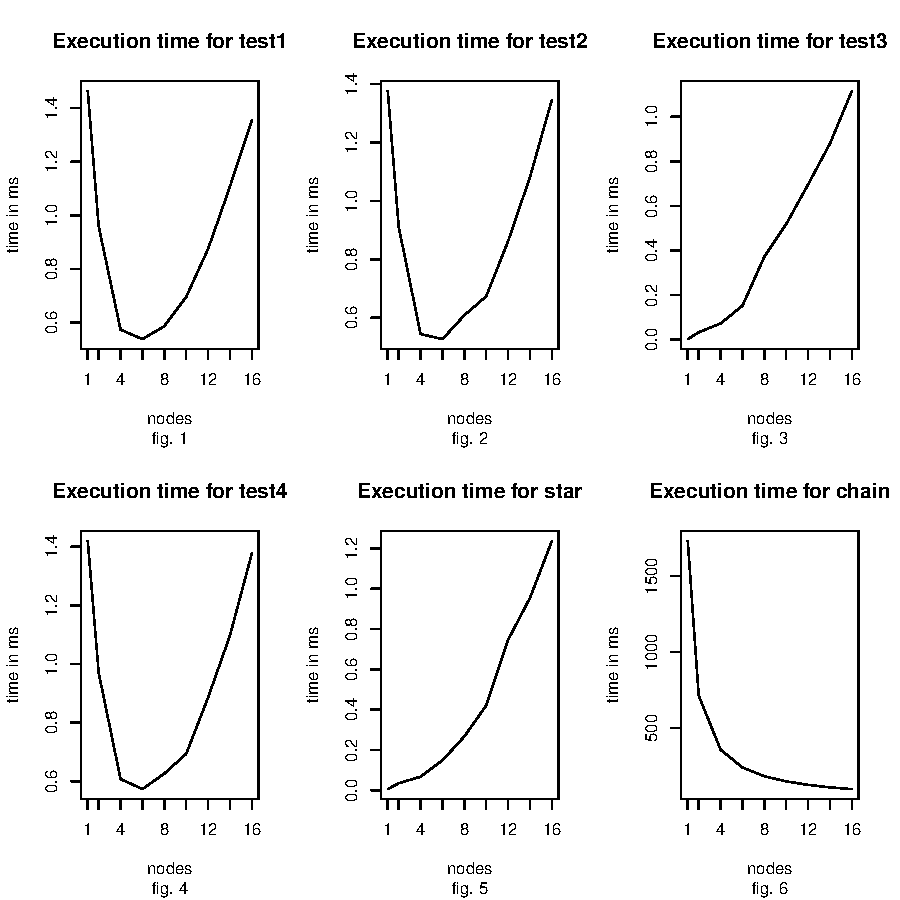
\includegraphics{report-001}

All tests were run on the DAS4 cluster computer. Each graph describes the execution time necessary for creating the shortest path matrix for all of the sample graphs provided. All tests were run using 1, 2, 4, 6, 8, 10, 12, 14, and 16 nodes. 

These graphs show the execution time of the algorithm taking each of the six provided sample graphs as input. What can be observed in the graphs for tests 1, 2 and 4 is that initially execution time drops as the number of nodes increases. After a certain point however, the execution time starts climbing. This can be explained by the fact that these are relatively small problems. Initially the parallelism provides a speedup. After a certain amount of nodes however, the communication overhead becomes larger than the benefit of parallelization. 

As for test 3 and Star, the problems were so small that communication overhead was instantly larger than any benefits provided by the parallel algorithm.

The chain test is the best example, showing a clear reduction in processing time as the number of nodes increases. This is also by far the largest problem, negating the negative impact of the required communication. We must note that because of restrictions on the DAS4 we were unable to run the sequential algorithm using this test file. We have decided to use a value obtained locally, using a 3.2Ghz AMD Quad Core (of which only one was used). The value from the DAS-server would probably be even higher, as the local machine is more powerful than a single node in the cluster. 

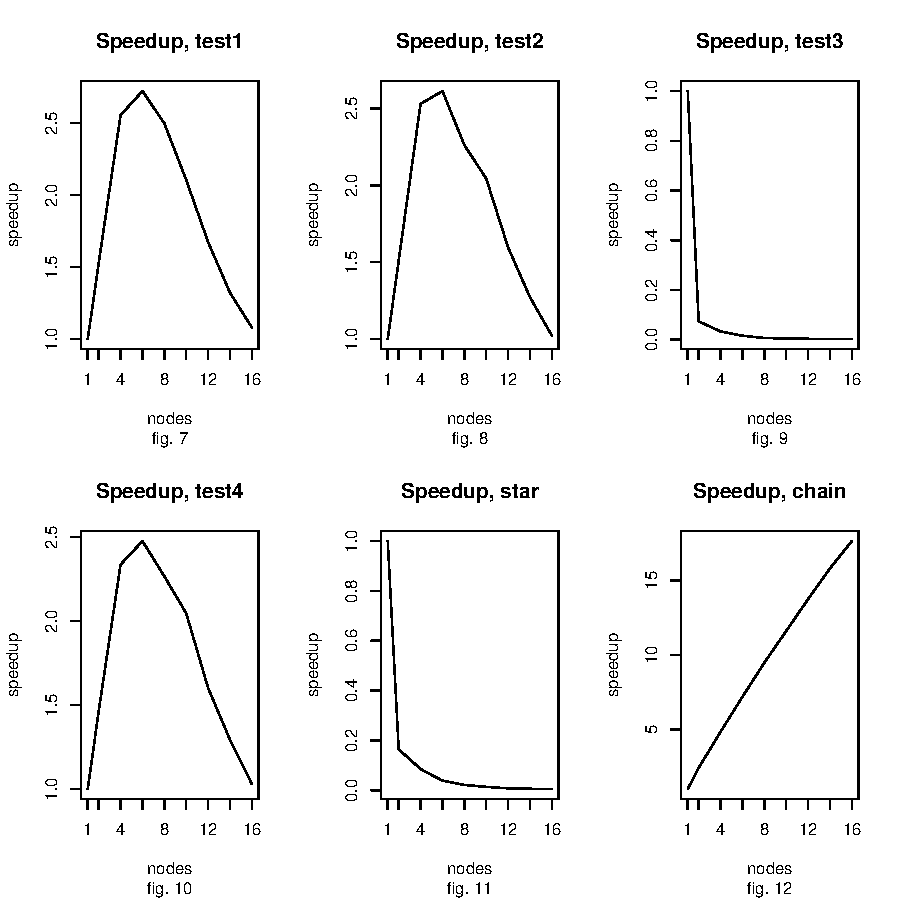
\includegraphics{report-002}

These graphs show the speedup achieved in comparison with running the sequential version. The explanation is much the same as with the execution time graphs: tests 1,2 and 4 get a slight boost initially, tests 3 and star are too small for any real speedups, and the chain test actually achieves near linear speedup. 

\section{Difficulties and Conclusion}

While implementing this algorithm we did not run into any real difficulties. The problem is straightforward and lends itself well to parallelization.

The conclusion we can draw from these experiments is that ASP lends itself very well to parallelization. It has limited use on small problems, as there is a substantial communication overhead, but it performs very well on large problems, achieving near linear speedup.


\end{document}
